\documentclass{article}

\usepackage[UTF8]{ctex}
\usepackage{amsmath}
\usepackage{graphicx,subfig}
\usepackage{caption}
\usepackage{booktabs}
\usepackage{indentfirst}
\setlength{\parindent}{2em}
\if CLASSOPTIONcompsoc
  \usepackage[nocompress]{cite}
\else
  % normal IEEE
  \usepackage{cite}
\fi



\title{语义分割记录}
\author{叶亮}
\date{\today}
\begin{document} 
\maketitle
\tableofcontents
\section{Basic mathematics}
\subsection{Normalization}
Batch Normalization:
\begin{align}
y = \frac{x - \mathrm{E}[x]}{ \sqrt{\mathrm{Var}[x] + \epsilon}} * \gamma + \beta \\
\hat{x}_\text{new} = (1 - \text{momentum}) \times \hat{x} + \text{momemtum} \times x_t
\end{align}

\subsection{Entropy}
信息熵:
\begin{align}
H(x) = -\sum_{x\in\chi}p(x)\log{p(x)} = \sum_{x\in\chi}p(x)\log{\dfrac{1}{{p(x)}}}
\end{align}
即事件发生概率的倒数的期望,熵越大代表事件发生的不可能性大,里面包含的信息量越大。

信息论解释:按照真实分布p来编码样本所需的编码长度的期望,信息熵$H(p)$.
\begin{align}
\sum_{i}p(i) * \log{\dfrac{1}{p(i)}}
\end{align}

交叉熵:按照不真实分布q来编码样本所需的编码长度的期望,$H(p,q)$
\begin{align}
\sum_{i}p(i) * \log{\dfrac{1}{q(i)}}
\end{align}

引申出KL散度$D(p||q) = H(p,q) - H(p)$,它也叫相对熵,表示两个分部的差异,差异越大,相对熵越大。
\begin{align}
\sum_{i}p(i) * \log{\dfrac{p(i)}{q(i)}} \\
D_KL(p||q) = \sum_{i=1}^{N}p(x_i) \cdot ( \log{p(x_i)}-\log{q(x_i)} )
\end{align}



\section{SF-segnet}
分割任务中影响性能的两个重要因素:分辨率和语义表征能力。常用的方法有:

atrous convolution:在后几个stage使用来保持高分辨率和较强的语义表征. 缺点:较大的计算能力和显存占用。

fpn-like network: 通过双边连接来融合low-level和high-level的特征,提高语义表征能力。

论文核心:fpn-like的连接方式ineffect.提出学习Semantic Flow between layers with different resolutions。即Flow Alignment Module(FAM),通过取相邻level的特征作为输入,输出offset field, and then warp the coarse feature to the fine feature with higher resolution according to the offset field. FAM为即插即用式,可插入到任意backbone中,called \textbf{SFNet}.灵感来源于光流。

在场景解析任务中,主要有两个范式(paradigm)用于高分辨率语义分割。1. 沿主路径keep spatial and semantic information. 2. distributes spatial and semantic information on different parts in a network, then merges back via different strategies.

The first is atrous convolution. The second is fuse multi-level feature maps for both spatiality and semantics

\subsection{Method}
文章采用了Encoder-decoder的架构。其中,Encoder部分为四个阶段的backbone,对应stage1, 2, 3, 4.步长分别为4, 8, 16, 32. Decoder部分为FPN的改进版。将之前的top-down部分的上采样相加模块替换成了Flow Alignment module(FAM). 通过语义流的方式来计算上采样的插值。在pytorch中的实现为:通过torch.grid{\_}sample来实现上采样差值运算。	

\section{DDRNet}
"Deep Dual-resolution Networks for Real-time and Accurate Semantic Segmentation of Road Scenes"\cite{hong2021deep}

Inspired by HRNet,作者使用双分支网络,如图所示:
\begin{figure}[htbp]
\centering
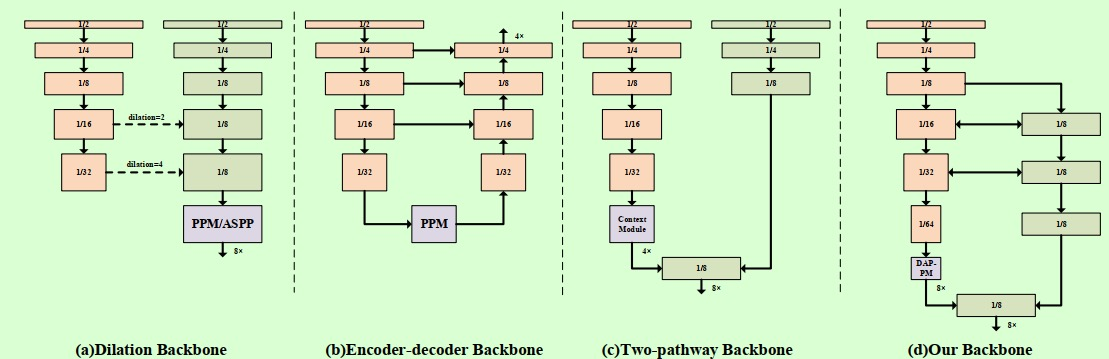
\includegraphics[scale=0.3]{image/DDR_arch.jpg}
\caption{不同架构的分割网络}
\label{Fig.ddr_arch}
\end{figure}
\subsection{相关工作}
\textbf{高性能分割}

大多数sota网络使用dilated backbone. Deeplabv3+使用更简单的decoder部分,通过将low-level和high-level的特征图融合进行预测,缓解了由dilated conv生成的高分辨率特征图的性能需求。HRNet则是通过更注重高分辨率特征表示。

\textbf{实时语义分割}

所有的实时语义分割方法采用两种基本的架构:encoder-decoder和two-pathway架构。

1) Encoder-decoder: 相比dilated convolution, encoder-decoder计算资源需求更少。通常encoder的输出步长为32,经过decoder逐渐上采样到1/4 or 1/8,且通常融合decoder和encoder的对应步长的特征图来提升表征能力。因此,其对显存的需求更少。

2) Two-pathway: encoder-decoder中的逐级下采样会损失partial information,且无法恢复。因此, two-pathway架构提出,通过在正常encoder之外,新建一个shallow pathway of high resolution来提供较丰富的空间信息。为了trade-off, two-pathway 可以是较轻的encoder和较宽的shallow branch. 在BiSeNet中,两个分支在一开始就进行分离。在Fast-SCNN中,两个分支使用相同的下采样。DDRNet则在早期使用相同的下采样,并在之后的stage中交换信息。

\subsection{Method}
\textbf{A Rethinking HRNet}
语义分割需要高分辨率特征图来做dense prediction,以及较大的感受野来解析场景。而多尺度表征能力,对目标检测任务更有意义,因为网络需要在一张图上尽可能多地对不同尺度的目标进行检测。因此,HRNet可以分为两个分支:1.用于维持高分辨率特征图; 2.用于生成较大感受野。本文通过优化,可以显著减少HRNet的显存消耗。

\textbf{B Dual-resolution for image classification}
主要介绍DDR的模型结构,包括DDR-23和DDR-39。两者分别使用Res-18和Res-34,通过修改开始的7x7conv为两个3x3 conv,使用双边连接模块来做特征融合。如图Fig .\ref{Fig.ddr_bilateral}
\begin{figure}
\centering
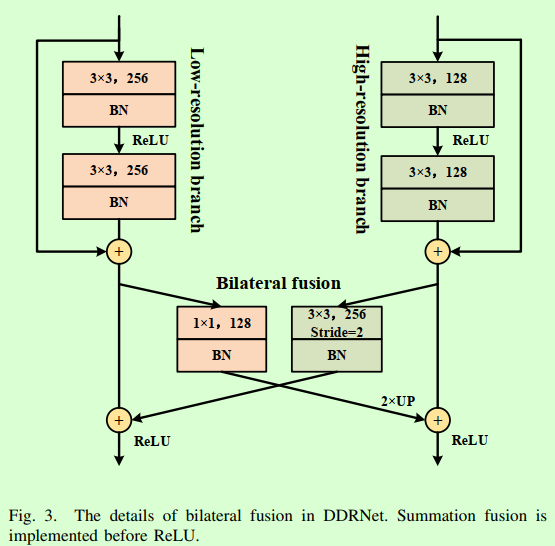
\includegraphics[scale=0.3]{image/DDR_bilateral.png}
\caption{bilateral融合}
\label{Fig.ddr_bilateral}
\end{figure}

\textbf{C Deep Aggregation Pyramid Pooling Module}
如图Fig .\ref{Fig.ddr_dappm}所示:
\begin{figure}
\centering
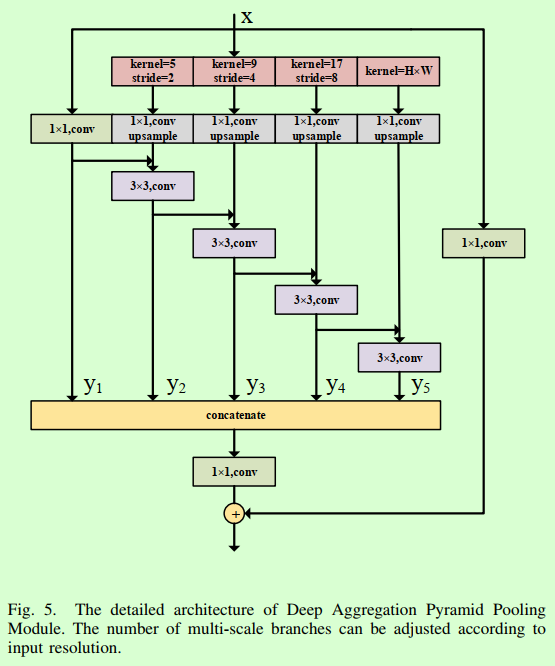
\includegraphics[scale=0.3]{image/DDR_dappm.png}
\caption{DAPPM}
\label{Fig.ddr_dappm}
\end{figure}

\textbf{D Overall architecture for Semantic Segmentation}
segmentaiton head channels set to 64,128,256 for DDR-23-slim, DDR-23, DDR-39.与其他方法一样,采用deep supervision方法,在stage 3的阶段加入auxiliary head,来辅助训练。如图Fig .\ref{Fig.ddr_arch2}所示:
\begin{figure}
\centering
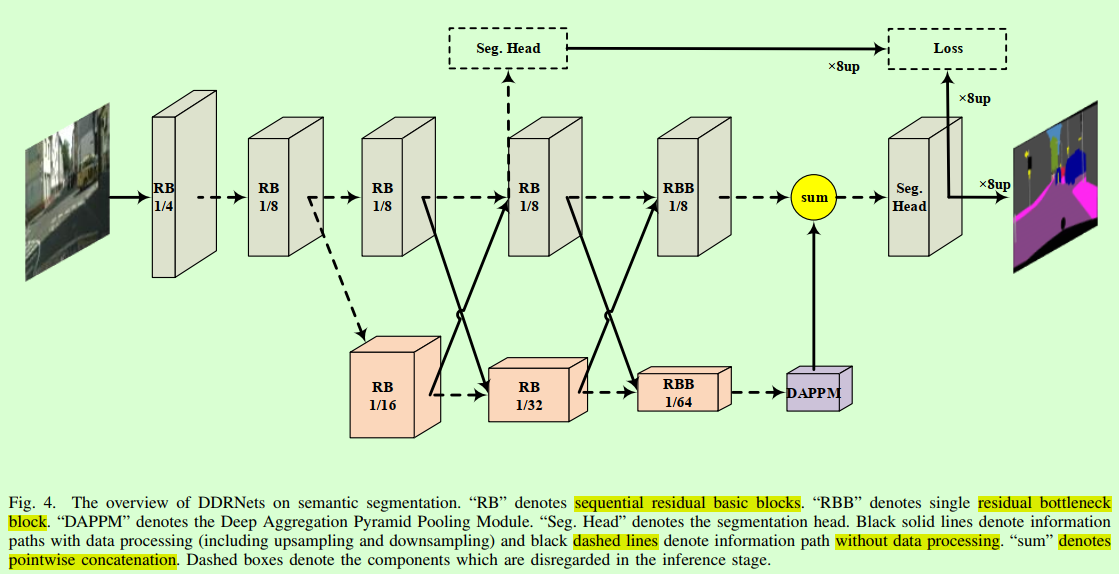
\includegraphics[scale=0.3]{image/DDR_arch2.png}
\caption{分割架构}
\label{Fig.ddr_arch2}
\end{figure}

\subsection{EMANet}
"Expectation-Maximization Attention Networks for Semantic Segmentation".

self-attention mechanism(自注意力机制),通过在特征图中所有位置加权求和的方式,来capture long-range relations.这篇论文中,将注意力机制表述成expectation-maximazation(期望最大化) manner 并iteratively estimate a much more compact set of bases upon which the attention maps are computed.主要贡献:
\begin{itemize}
\item 将自注意机制定义为EM iteration manner,which can learn a more compact basis set and largely reduce the computational complexity.
\item proposed EMA module and set up specific manners for bases' maintenance and normalization.
\item Extensive experiments
\end{itemize}

\subsection{相关工作与知识点}
\subsubsection{Expectation-Maximization Algorithm}
EM aims to find the maximum likelihood solution for latent variable models. Denote $X={x_1,x_2,...,x_N}	$ 作为观测样本,每个$x_i$有对应的latent variable$z_i$. 将${X,Z}$表示完整数据(complete data),似然函数的形式为$\ln p(X,Z|\theta)$, where $\theta$表示模型的所有参数。latent variable $Z$ is given by后验分布$p(Z|X,\theta)$. EM算法通过两步来最大化似然函数$\ln p(X,Z|\theta)$, i.e., E and M.



\bibliographystyle{IEEEtran}
\bibliography{reference.bib}

\end{document}


